\section{process creation and management}

\begin{frame}<1>[label=posixProcessFunctions]{POSIX process management}
\begin{itemize}
\item essential operations
\vspace{.5cm}
\item process information: \myemph<2>{\texttt{getpid}}
\item process creation: \myemph<3>{\texttt{fork}}
\item running programs: \myemph<4>{\texttt{exec*}}
\begin{itemize}
\item {\fontsize{9}{10}\selectfont also \texttt{posix\_spawn} (not widely supported), \ldots}
\end{itemize}
\item waiting for processes to finish: \texttt{\myemph<5>{waitpid}} {\small (or \texttt{\myemph<5>{wait}})}
\item process destruction, `signaling': \texttt{exit}, \texttt{kill}
\end{itemize}
\end{frame}



\againframe<3>{posixProcessFunctions}


\usetikzlibrary{matrix,patterns,arrows.meta,decorations.pathreplacing}
\begin{frame}{\texttt{fork}}
\begin{itemize}
\item \texttt{pid\_t fork()} --- copy the current process
\item returns twice:
    \begin{itemize}
    \item in \textit{parent} (original process): pid of new \textit{child} process
    \item in \textit{child} (new process): \texttt{0}
    \end{itemize}
\item \myemph{everything (but pid) duplicated} in parent, child:
    \begin{itemize}
    \item memory
    \item file descriptors (later)
    \item registers
    \end{itemize}
\end{itemize}
\end{frame}


\usetikzlibrary{matrix,patterns,arrows.meta,decorations.pathreplacing}

% FIXME: fork process control block image

\begin{frame}[label=forkPCBs]{fork and process info (w/o copy-on-write)}
\begin{tikzpicture}
\tikzset{
    pcb/.style={
        tight matrix,
        column 1/.style={nodes={draw,thin,text width=3.0cm,font=\small,minimum height=0.4cm}},
        column 2/.style={nodes={draw,thin,text width=5.5cm,font=\fontsize{9}{10}\tt\selectfont,minimum height=0.4cm}},
    },
    page/.style={
        draw,thick,
        pattern=north west lines,
        minimum width=2cm,
        node contents={~},
    },
    pointer/.style={
        draw,very thick,-Latex,
    },
    pointer light/.style={
        draw,thick,-Latex,
    },
    tall/.style={
        minimum height=0.85cm
    },
    one pt/.style={
        fill=blue!40,
    },
    one pt line/.style={
        draw=blue!80!black,
    },
    one memory/.style={
        fill=green!40,
    },
    one memory line/.style={
        draw=green!80!black,
    },
    two pt/.style={
        fill=orange!40,
    },
    two pt line/.style={
        draw=orange!80!black,
    },
    two memory/.style={
        fill=violet!40,
        alt=<1-2>{one memory},
    },
    two memory line/.style={
        draw=violet!80!black,
        alt=<1-2>{one memory line},
    },
    fork line/.style={
        draw=black!30,line width=2mm,-{Latex[length=6mm]}
    },
}
\matrix[pcb,label={[font=\small]north:parent process info}] (proc one) {
    |[tall]| user regs \&
    |[tall]|
    {rax {\fontsize{8}{9}\selectfont (return val.)}=\sout<5->{42}\only<5->{\textit{\myemph<5>{child pid}}}, \\ rcx=133,} \ldots \\
    memory mapping \& |[one pt]| ~ \\
    |[tall]| open files \& |[tall]| {fd 0: \ldots \\ fd 1: \ldots } \\
    \ldots \& \ldots \\
};
\newcommand{\halfvthick}{.2mm}
\node[draw,very thick,pattern=north west lines,minimum width=2cm,minimum height=6cm,anchor=north west,
    label={north:memory}] (memory) at ([xshift=1.5cm,yshift=0cm]proc one.north east) {};
\foreach \y in {-1.8cm} {
    \draw[very thick,one pt] ([yshift=\y,xshift=\halfvthick]memory.north west) rectangle ++ (2cm,-1mm);
}
\coordinate (one pt root) at ([yshift=-1.8cm-0.5mm,xshift=\halfvthick]memory.north west);
\draw[pointer light,one pt line] (proc one-2-2.east) -- ++(.25cm,0cm) |- ([yshift=-1.8cm]memory.north west);
\draw[pointer light,one memory line] (one pt root) -- ++(-.5cm,0cm) |- ([yshift=-0.9cm]memory.north west);
\draw[pointer light,one memory line] (one pt root) -- ++(-.5cm,0cm) |- ([yshift=-1.1cm]memory.north west);
\draw[pointer light,one memory line] (one pt root) -- ++(-.5cm,0cm) |- ([yshift=-1.5cm]memory.north west);
\foreach \y in {-0.9cm,-1.1cm,-1.5cm} {
    \draw[very thick,one memory] ([yshift=\y,xshift=\halfvthick]memory.north west) rectangle ++ (2cm,-1mm);
}
\begin{visibleenv}<2->
\matrix[pcb,anchor=north west,label={[font=\small]north:child process info}] (proc two) at ([yshift=-1cm]proc one.south west) {
    |[tall]| user regs \&
    |[tall]|
    {rax {\fontsize{8}{9}\selectfont(return val.)}=\sout<5->{42}\only<5->{\myemph<5>{0}}, \\ rcx=133, \ldots} \\
    memory mapping \& |[two pt]| ~ \\
    |[tall]| open files \& |[tall]| {fd 0: \ldots \\ fd 1: \ldots } \\
    \ldots \& \ldots \\
};
\draw[fork line] ([xshift=-0.25cm]proc one.west) -- ++(-1cm,0cm) |- ([xshift=-0.25cm]proc two.west)
    node[pos=0.25,right] {copy};
\end{visibleenv}
\begin{visibleenv}<3->
\foreach \y in {-4.3cm} {
    \draw[very thick,two pt] ([yshift=\y,xshift=\halfvthick]memory.north west) rectangle ++ (2cm,-1mm);
}
\coordinate (two pt root) at ([yshift=-4.3cm-0.5mm,xshift=\halfvthick]memory.north west);
\draw[pointer light,two pt line] (proc two-2-2.east) -- ++(.25cm,0cm) |- ([yshift=-4.3cm]memory.north west);
\draw[pointer light,two memory line] (two pt root) -- ++(-.75cm,0cm) |- ([yshift=-4.4cm]memory.north west);
\draw[pointer light,two memory line] (two pt root) -- ++(-.75cm,0cm) |- ([yshift=-4.6cm]memory.north west);
\draw[pointer light,two memory line] (two pt root) -- ++(-.75cm,0cm) |- ([yshift=-4.7cm]memory.north west);
\foreach \y in {-4.4cm,-4.6cm,-4.7cm} {
    \draw[very thick,two memory] ([yshift=\y,xshift=\halfvthick]memory.north west) rectangle ++ (2cm,-1mm);
}
\draw[fork line] ([yshift=-1.4cm,xshift=.5cm]memory.north east) coordinate (one memory)-- ++(1cm, 0cm) |- ([yshift=-4.6cm,xshift=.5cm]memory.north east) coordinate (two memory)
    node[pos=0.25,left] {copy};
\draw[ultra thick,decorate,decoration={brace,mirror}] ([xshift=-.25cm,yshift=-6mm]one memory) -- ([xshift=-.25cm,yshift=6mm]one memory);
\draw[ultra thick,decorate,decoration={brace,mirror}] ([xshift=-.25cm,yshift=-6mm]two memory) -- ([xshift=-.25cm,yshift=6mm]two memory);
\end{visibleenv}
\end{tikzpicture}
\end{frame}

%\usetikzlibrary{matrix,patterns,arrows.meta,decorations.pathreplacing}

\begin{frame}[label=forkCows]{fork (w/ copy-on-write, if parent writes first)}
\begin{tikzpicture}
\tikzset{
    pcb/.style={
        tight matrix,
        column 1/.style={nodes={draw,thin,text width=2.5cm,font=\small,minimum height=0.4cm}},
        column 2/.style={nodes={draw,thin,text width=5.5cm,font=\fontsize{9}{10}\tt\selectfont,minimum height=0.4cm}},
    },
    page/.style={
        draw,thick,
        pattern=north west lines,
        minimum width=2cm,
        node contents={~},
    },
    pointer/.style={
        draw,very thick,-Latex,
    },
    pointer light/.style={
        draw,thick,-Latex,
    },
    tall/.style={
        minimum height=0.85cm
    },
    one pt/.style={
        fill=blue!40,
    },
    one pt line/.style={
        draw=blue!80!black,
    },
    one memory/.style={
        fill=green!40,
    },
    shared memory/.style={
        fill=yellow!40,
    },
    one memory line/.style={
        draw=green!80!black,
    },
    one memory line cow/.style={
        draw=green!80!black,
        dashed,
    },
    two pt/.style={
        fill=orange!40,
    },
    two pt line/.style={
        draw=orange!80!black,
    },
    two memory/.style={
        fill=violet!40,
    },
    two memory line/.style={
        draw=violet!80!black,
    },
    two memory line cow/.style={
        draw=violet!80!black,
        dashed 
    },
    fork line/.style={
        draw=black!30,line width=2mm,-{Latex[length=6mm]}
    },
}
\matrix[pcb,label={[font=\small]north:parent process info}] (proc one) {
    |[tall]| user regs \&
    |[tall]|
    {rax {\fontsize{8}{9}\selectfont (return val.)}=\sout<1->{42}\only<1->{\textit{\myemph<5>{child pid}}}, \\ rcx=133,} \ldots \\
    page tables \& |[one pt]| ~ \\
    |[tall]| open files \& |[tall]| {fd 0: \ldots \\ fd 1: \ldots } \\
    \ldots \& \ldots \\
};
\newcommand{\halfvthick}{.2mm}
\node[draw,very thick,pattern=north west lines,minimum width=2cm,minimum height=6cm,anchor=north west,
    label={north:memory}] (memory) at ([xshift=1.5cm,yshift=0cm]proc one.north east) {};
\foreach \y in {-1.8cm} {
    \draw[very thick,one pt] ([yshift=\y,xshift=\halfvthick]memory.north west) rectangle ++ (2cm,-1mm);
}
\coordinate (one pt root) at ([yshift=-1.8cm-0.7mm,xshift=\halfvthick]memory.north west);
\draw[pointer light,one pt line] (proc one-2-2.east) -- ++(.25cm,0cm) |- ([yshift=-1.8cm]memory.north west);
\begin{visibleenv}<1>
\draw[pointer light,one memory line] (one pt root) -- ++(-.5cm,0cm) |- ([yshift=-0.4cm]memory.north west);
\draw[pointer light,one memory line] (one pt root) -- ++(-.6cm,0cm) |- ([yshift=-1.1cm]memory.north west);
\draw[pointer light,one memory line] (one pt root) -- ++(-.7cm,0cm) |- ([yshift=-1.5cm]memory.north west);
\end{visibleenv}
\begin{visibleenv}<2>
\draw[pointer light,one memory line cow] (one pt root) -- ++(-.5cm,0cm) |- ([yshift=-0.4cm]memory.north west);
\end{visibleenv}
\begin{visibleenv}<3->
\draw[pointer light,one memory line,alt=<3>{red,very thick}] (one pt root) -- ++(-.5cm,0cm) |- ([yshift=-2.9cm]memory.north west);
\end{visibleenv}
\begin{visibleenv}<2->
\draw[pointer light,one memory line cow] (one pt root) -- ++(-.6cm,0cm) |- ([yshift=-1.1cm]memory.north west);
\draw[pointer light,one memory line cow] (one pt root) -- ++(-.7cm,0cm) |- ([yshift=-1.5cm]memory.north west);
\end{visibleenv}
\begin{visibleenv}<1>
\foreach \y in {-0.4cm,-1.1cm,-1.5cm} {
    \draw[very thick,one memory] ([yshift=\y,xshift=\halfvthick]memory.north west) rectangle ++ (2cm,-1mm);
}
\end{visibleenv}
\begin{visibleenv}<2->
\foreach \y in {-0.4cm,-1.1cm,-1.5cm} {
    \draw[very thick,shared memory] ([yshift=\y,xshift=\halfvthick]memory.north west) rectangle ++ (2cm,-1mm);
}
\end{visibleenv}
\begin{visibleenv}<2>
\path ([yshift=-0.8cm,xshift=0cm]memory.north east) coordinate (base memory) node [right=0.5mm,align=left] {shared\\read-only};
\draw[ultra thick,decorate,decoration={brace,mirror}] ([xshift=.1cm,yshift=-7mm]base memory) -- ([xshift=.1cm,yshift=7mm]base memory);
\end{visibleenv}
\begin{visibleenv}<3-4>
\path ([yshift=-1.3cm,xshift=0cm]memory.north east) coordinate (base memory alt) node [right=0.5mm,align=left] {shared\\read-only};
\draw[ultra thick,decorate,decoration={brace,mirror}] ([xshift=.1cm,yshift=-3mm]base memory alt) -- ([xshift=.1cm,yshift=3mm]base memory alt);
\end{visibleenv}
\begin{visibleenv}<3->
\foreach \y in {-2.9cm} {
    \draw[very thick,one memory] ([yshift=\y,xshift=\halfvthick]memory.north west) rectangle ++ (2cm,-1mm);
}
\path[alt=<3>{red}] ([yshift=-2.9cm,xshift=0cm]memory.north east) coordinate (copied memory) node [inner sep=0mm,right=4mm,align=left] (copy label) {copied};
    \node[align=left,font=\small,anchor=north west,inner sep=0.5mm] at (copy label.south west) {for\\ parent's\\ write};
\draw[ultra thick,decorate,decoration={brace,mirror}] ([xshift=.1cm,yshift=-2mm]copied memory) -- ([xshift=.1cm,yshift=2mm]copied memory);
\end{visibleenv}
\begin{visibleenv}<4>
\path[alt=<4>{red}] ([yshift=-0.4cm,xshift=0cm]memory.north east) coordinate (now unshared memory) node[inner sep=0mm,right=0mm]{$\leftarrow$} node [inner sep=0mm,right=5mm,align=left,font=\small] {no longer\\shared};
\draw[ultra thick,decorate,decoration={brace,mirror}] ([xshift=.1cm,yshift=-2mm]copied memory) -- ([xshift=.1cm,yshift=2mm]copied memory);
\end{visibleenv}
\begin{visibleenv}<3>
\path[alt=<3>{red}] ([yshift=-0.4cm,xshift=0cm]memory.north east) coordinate (uncopied memory) node[inner sep=0mm,right=0mm]{$\leftarrow$} node [inner sep=0mm,right=5mm,align=left,font=\small] {on parent\\write};
\end{visibleenv}
\begin{visibleenv}<2->
\matrix[pcb,anchor=north west,label={[font=\small]north:child process info}] (proc two) at ([yshift=-1cm]proc one.south west) {
    |[tall]| user regs \&
    |[tall]|
    {rax {\fontsize{8}{9}\selectfont(return val.)}=\sout<1->{42}\only<1->{\myemph<5>{0}}, \\ rcx=133, \ldots} \\
    page tables\& |[two pt]| ~ \\
    |[tall]| open files \& |[tall]| {fd 0: \ldots \\ fd 1: \ldots } \\
    \ldots \& \ldots \\
};
\draw[fork line] ([xshift=-0.25cm]proc one.west) -- ++(-1cm,0cm) |- ([xshift=-0.25cm]proc two.west)
    node[pos=0.25,right] {copy};
\end{visibleenv}
\begin{visibleenv}<2->
\foreach \y in {-4.3cm} {
    \draw[very thick,two pt] ([yshift=\y,xshift=\halfvthick]memory.north west) rectangle ++ (2cm,-1mm);
}
\coordinate (two pt root) at ([yshift=-4.3cm-0.5mm,xshift=\halfvthick]memory.north west);
\draw[pointer light,two pt line] (proc two-2-2.east) -- ++(.25cm,0cm) |- ([yshift=-4.3cm]memory.north west);
\begin{visibleenv}<2->
\draw[pointer light,two memory line cow] (two pt root) -- ++(-.75cm,0cm) |- ([yshift=-0.45cm]memory.north west);
\draw[pointer light,two memory line cow] (two pt root) -- ++(-.75cm,0cm) |- ([yshift=-1.15cm]memory.north west);
\draw[pointer light,two memory line cow] (two pt root) -- ++(-.75cm,0cm) |- ([yshift=-1.55cm]memory.north west);
\end{visibleenv}
\begin{visibleenv}<0>
\draw[pointer light,two memory line] (two pt root) -- ++(-.75cm,0cm) |- ([yshift=-4.4cm]memory.north west);
\draw[pointer light,two memory line] (two pt root) -- ++(-.75cm,0cm) |- ([yshift=-4.6cm]memory.north west);
\draw[pointer light,two memory line] (two pt root) -- ++(-.75cm,0cm) |- ([yshift=-4.7cm]memory.north west);
\end{visibleenv}
\begin{visibleenv}<0>
\foreach \y in {-4.4cm,-4.6cm,-4.7cm} {
    \draw[very thick,two memory] ([yshift=\y,xshift=\halfvthick]memory.north west) rectangle ++ (2cm,-1mm);
}
\end{visibleenv}
% FIXME: XXX -----> = read-only marker
%\draw[fork line] ([yshift=-1.4cm,xshift=.5cm]memory.north east) coordinate (one memory)-- ++(1cm, 0cm) |- ([yshift=-4.6cm,xshift=.5cm]memory.north east) coordinate (two memory)
%    node[pos=0.25,left] {copy};
%\draw[ultra thick,decorate,decoration={brace,mirror}] ([xshift=-.25cm,yshift=-6mm]one memory) -- ([xshift=-.25cm,yshift=6mm]one memory);
%\draw[ultra thick,decorate,decoration={brace,mirror}] ([xshift=-.25cm,yshift=-6mm]two memory) -- ([xshift=-.25cm,yshift=6mm]two memory);
\end{visibleenv}
\end{tikzpicture}
\end{frame}
 % in backup

\begin{frame}{fork example}
\lstinputlisting[
    language=C,
    basicstyle=\sourcecodepro\fontsize{9}{10}\selectfont,
    moredelim={**[is][\btHL<2|handout:0>]{@2}{2@}},
    moredelim={**[is][\btHL<3|handout:0>]{@3}{3@}},
    moredelim={**[is][\btHL<4|handout:0>]{@4}{4@}},
]{../unix-api/fork1.c}
\begin{tikzpicture}[overlay,remember picture]
\coordinate (explain location) at ([xshift=-1cm,yshift=-2cm]current page.north east);
\tikzset{
    explain box/.style={
        at={(explain location)},
        anchor=north east,
        draw=red,
        very thick,
        align=left,
        fill=white
    },
}
\begin{visibleenv}<2|handout:0>
\node[explain box] {
\texttt{getpid} --- returns current process pid
};
\end{visibleenv}
\begin{visibleenv}<3|handout:0>
\node[explain box] {
cast in case \texttt{pid\_t} isn't int \\
POSIX doesn't specify (some systems it is, some not\ldots) \\
(not necessary if you were using C++'s cout, etc.)
};
\end{visibleenv}
\begin{visibleenv}<4|handout:0>
\node[explain box] {
prints out \texttt{Fork failed: \textit{error message}} \\
(example \textit{error message}: ``Resource temporarily unavailable'') \\
from error number stored in special global variable \texttt{errno} 
};
\end{visibleenv}
\begin{visibleenv}<5|handout:2>
\node[explain box] {
Example output: \\
\texttt{Parent pid: 100} \\
\texttt{[100] parent of [432]} \\
\texttt{[432] child}
};
\end{visibleenv}
\end{tikzpicture}
\end{frame}


% FIXME: fork_race.c?

% Other process management




\begin{frame}[fragile,label=forkQuestion]{a fork question}
\vspace{-.3cm}
\begin{lstlisting}[language=C++,style=size10]
int main() {
    pid_t pid = fork();
    if (pid == 0) {
        printf("In child\n");
    } else {
        printf("Child %d\n", pid);
    }
    printf("Done!\n");
}
\end{lstlisting}
\tikzmark{question start}\small Exercise: Suppose the pid of the parent process is \texttt{99} and child is \texttt{100}. Give \textbf{two} possible outputs. (Assume no crashes, etc.)
\begin{tikzpicture}[overlay,remember picture]
\coordinate (timeline start) at ([yshift=-2cm]pic cs:question start);
\tikzset{
    prog1/.style={draw,fill=cyan},
    prog2/.style={draw,fill=green},
    proglabel/.style={font=\tt\scriptsize},
    labelprog1/.style={execute at begin node={\strut parent}},
    labelprog2/.style={execute at begin node={\strut child}},
}
\iftoggle{heldback}{}{
\begin{visibleenv}<2>
\begin{scope}[shift={(timeline start)}]
\begin{scope}[xscale=1.5,yscale=0.9]
    % FIXME: more suggestive split
\foreach \s/\e/\p [count=\x] in {0/1.5/1,1.5/3/2,3/4.5/1,4.5/5.5/2,5.5/7/1}{
    \coordinate (s-\x) at (\s, 0);
    \coordinate (e-\x) at (\e, 0);
    \draw[prog\p] (\s, 0) rectangle (\e, 1) coordinate[midway] (mid-\x);
    \node[anchor=center,proglabel,labelprog\p] at (mid-\x) {};
    \draw[fill=white] ([xshift=-.05cm]e-\x) rectangle ([xshift=.05cm,yshift=1cm]e-\x);
    \draw[pattern=north west lines] ([xshift=-.05cm]e-\x) rectangle ([xshift=.05cm,yshift=1cm]e-\x);
}
\node[overlay,anchor=west,font=\tt\fontsize{9}{10}\selectfont,align=left] at (7.5, .8) { Child 100 \\ In child \\ Done! \\ Done!};
\begin{scope}[yshift=-1.5cm]
\foreach \s/\e/\p [count=\x] in {0/1/1,1/4/2,4/7/1}{
    \coordinate (s-\x) at (\s, 0);
    \coordinate (e-\x) at (\e, 0);
    \draw[prog\p] (\s, 0) rectangle (\e, 1) coordinate[midway] (mid-\x);
    \node[anchor=center,proglabel,labelprog\p] at (mid-\x) {};
    \draw[fill=white] ([xshift=-.05cm]e-\x) rectangle ([xshift=.05cm,yshift=1cm]e-\x);
    \draw[pattern=north west lines] ([xshift=-.05cm]e-\x) rectangle ([xshift=.05cm,yshift=1cm]e-\x);
}
\node[anchor=west,font=\tt\fontsize{9}{10}\selectfont,align=left] at (7.5, .5) { In child \\ Done! \\ Child 100 \\ Done! };
\end{scope}
\end{scope}
\end{scope}
\end{visibleenv}
}
\end{tikzpicture}
\end{frame}


\subsection{exec}

\againframe<4>{posixProcessFunctions}

\usetikzlibrary{matrix,patterns,arrows.meta,decorations.pathreplacing,shapes.misc,fit}

\begin{frame}{exec*}
\begin{itemize}
\item exec* --- \myemph{replace} current program with new program
    \begin{itemize}
    \item * --- multiple variants
    \item same pid, new process image
    \end{itemize}
\item \texttt{int execv(const char *path, const char **argv)}
    \begin{itemize}
    \item path: new program to run
    \item argv: array of arguments, termianted by null pointer
    \end{itemize}
\end{itemize}
\end{frame}

\begin{frame}[fragile,label=execExample1]{execv example}
\begin{lstlisting}[
    language=C++,
    style=small,
    moredelim={**[is][\btHL<2|handout:0>]{@2}{2@}},
    moredelim={**[is][\btHL<3|handout:0>]{@3}{3@}},
    moredelim={**[is][\btHL<4|handout:0>]{@4}{4@}},
]
  ...
  child_pid = fork();
  if (child_pid == 0) {
    /* child process */
    char *args[] = @2{"ls", "-l", NULL}2@;
    execv(@3"/bin/ls"3@, @2args2@);
    /* execv doesn't return when it works.
       So, if we got here, it failed. */
    perror("execv");
    exit(1);
  } else if (child_pid > 0) {
    /* parent process */
    ...
  }
\end{lstlisting}
\begin{tikzpicture}[overlay,remember picture]
\coordinate (explain location) at ([xshift=-1cm,yshift=-5cm]current page.north east);
\tikzset{
    explain box/.style={
        at={(explain location)},
        anchor=north east,
        draw=red,
        very thick,
        align=left,
        fill=white
    },
}
\begin{visibleenv}<2|handout:0>
\node[explain box] {
used to compute argv, argc \\
when program's \texttt{main} is run \\
~ \\
convention: first argument is program name
};
\end{visibleenv}
\begin{visibleenv}<3|handout:0>
\node[explain box] {
path of executable to run \\
need not match first argument \\
(but probably should match it) \\
~  \\
on Unix {\texttt /bin} is a directory \\
containing many common programs, \\
including \texttt{ls} (`list directory')
};
\end{visibleenv}
\end{tikzpicture}
\end{frame}


\usetikzlibrary{fit,arrows.meta,matrix,decorations.pathreplacing,shapes.misc}

\begin{frame}{exec in the kernel}
\begin{tikzpicture}
\tikzset{
    pcb/.style={
        tight matrix,
        column 1/.style={nodes={draw,thin,text width=3cm,font=\small,minimum height=0.4cm}},
        column 2/.style={nodes={draw,thin,text width=4cm,font=\fontsize{9}{10}\tt\selectfont,minimum height=0.4cm}},
    },
    page/.style={
        draw,thick,
        pattern=north west lines,
        minimum width=2cm,
        node contents={~},
    },
    pointer/.style={
        draw,very thick,-Latex,
    },
    pointer light/.style={
        draw,thick,-Latex,
    },
    tall/.style={
        minimum height=0.85cm
    },
    one pt/.style={
        fill=blue!40,
    },
    one pt line/.style={
        draw=blue!80!black,
    },
    one memory/.style={
        fill=green!40,
    },
    one memory line/.style={
        draw=green!80!black,
        alt=<2->{opacity=0.2,dotted},
    },
    two memory/.style={
        fill=violet!40,
        alt=<2>{draw=red,thick},
    },
    two memory line/.style={
        draw=violet!80!black,
    },
    mark line/.style={
        draw,thick,Latex-,
    },
    mark line reversed/.style={
        draw,thick,-Latex,
    }
}
\matrix[pcb,label={[font=\small]north:the process control block}] (proc one) {
    |[tall]| user regs \&
    |[tall]|
    {eax=\sout<2->{42}{\normalfont\it \only<2->{\myemph<2>{init. val.}}}, \\ ecx=\sout<2->{133}\only<2->{\normalfont\it \myemph<2>{init. val.}},} \ldots \\
    memory mapping\& |[one pt]| ~ \\
    |[tall]| open files \& |[tall,alt=<4>{red,thick},alias=fds]| {fd 0: (terminal \ldots) \\ fd 1: \ldots } \\
    \ldots \& \ldots \\
};
\newcommand{\halfvthick}{.2mm}
\node[draw,very thick,pattern=north west lines,minimum width=2cm,minimum height=6cm,anchor=north west,
    label={north:memory}] (memory) at ([xshift=3cm,yshift=0cm]proc one.north east) {};
\draw[pointer,one pt line] (proc one-2-2.east) -- ++(.5cm,0cm) |- ([yshift=-1.8cm]memory.north west) coordinate (one pt base);
\foreach \y in {-1.8cm} {
    \draw[very thick,one pt] ([yshift=\y,xshift=\halfvthick]memory.north west) rectangle ++ (2cm,-1mm);
}
\draw[pointer light,one memory line] ([yshift=-.2mm]one pt base) -- ++(-.5cm,0cm) |- ([yshift=-0.9cm]memory.north west);
\draw[pointer light,one memory line] ([yshift=-.1mm]one pt base) -- ++(-.6cm,0cm) |- ([yshift=-1.1cm]memory.north west) coordinate (args memory);
\draw[pointer light,one memory line] ([yshift=.1mm]one pt base) -- ++(-.7cm,0cm) |- ([yshift=-1.5cm]memory.north west);
\foreach \y/\v in {-0.9cm/A,-1.1cm/B,-1.5cm/C} {
    \draw[very thick,one memory] ([yshift=\y,xshift=\halfvthick]memory.north west) coordinate (orig-\v) rectangle ++ (2cm,-1mm) coordinate (orig-other-\v);
}
\begin{visibleenv}<2->
\draw[pointer light,two memory line] ([yshift=-.1mm]one pt base) -- ++(-.5cm,0cm) |- ([yshift=-4.4cm]memory.north west);
\draw[pointer light,two memory line] ([yshift=-.2mm]one pt base) -- ++(-.6cm,0cm) |- ([yshift=-4.6cm]memory.north west);
\draw[pointer light,two memory line] ([yshift=-.3mm]one pt base) -- ++(-.7cm,0cm) |- ([yshift=-5cm]memory.north west);
\draw[pointer light,two memory line] ([yshift=-.4mm]one pt base) -- ++(-.8cm,0cm) |- ([yshift=-5.1cm]memory.north west);
\foreach \y in {-4.4cm,-4.6cm,-5cm,-5.1cm} {
    \draw[very thick,two memory] ([yshift=\y,xshift=\halfvthick]memory.north west) rectangle ++ (2cm,-1mm);
}
\draw[mark line] ([yshift=-5.15cm]memory.north east) -| ++(2cm,-.5cm) node[below,align=center,font=\small] { \myemph<2>{loaded from} \\ \myemph<2>{executable file} };
\coordinate (new memory) at ([yshift=-4.7cm,xshift=.25cm]memory.north east);
\draw[ultra thick,decorate,decoration={brace,mirror}] ([xshift=-.15cm,yshift=-3mm]new memory) -- ([xshift=-.15cm,yshift=3mm]new memory);
\node[anchor=west,font=\small] (new stack text) at ([xshift=-1.5mm]new memory) { \myemph<2>{new stack, heap, \ldots} };
\end{visibleenv}
\begin{visibleenv}<3->
\draw[mark line reversed] ([xshift=2cm]args memory) -| (new stack text.north) node[pos=0.75,fill=white,font=\small] {\myemph<3>{copy arguments}};
\end{visibleenv}
\begin{visibleenv}<4->
    \draw[mark line,alt=<4>{draw=red}{blue},ultra thick] (fds.south) -- ++(0cm, -2cm) node[below,align=center] { files + some other things not changed! \\ (more on this later) };
\end{visibleenv}
\begin{visibleenv}<5>
\node[cross out,draw=red,very thick,fit=(orig-A) (orig-other-C),label={[align=center,red]north east:old memory\\discarded}] {};
\end{visibleenv}
\end{tikzpicture}
\end{frame}


\subsection{aside: fork+exec, really?}

\begin{frame}{why fork/exec?}
    \begin{itemize}
    \item could just have a function to spawn a new program
        \begin{itemize}
        \item Windows \texttt{CreateProcess()}; POSIX's (rarely used) \texttt{posix\_spawn}
        \end{itemize}
    \vspace{.5cm}
    \item some other OSs do this (e.g. Windows)
    \item needs to include API to set new program's state
        \begin{itemize}
        \item e.g. without fork: either: \\
        need function to set new program's current directory, \textit{or} \\
        need to change your directory, then start program, then change back
        \item e.g. with fork: just change your current directory before exec
        \end{itemize}
    \item but allows OS to avoid `copy everything' code
        \begin{itemize}
        \item probably makes OS implementation easier
        \end{itemize}
    \end{itemize}
\end{frame}

\begin{frame}[fragile,label=posixSpawn]{posix\_spawn}
\begin{lstlisting}[style=small]
pid_t new_pid;
const char argv[] = { "ls", "-l", NULL };
int error_code = posix_spawn(
    &new_pid,
    "/bin/ls",
    NULL /* null = copy current process's open files;
            if not null, do something else */,
    NULL /* null = no special settings for new process */,
    argv,
    NULL /* null = copy current "environment variables", 
            if not null, do something else */
);
if (error_code == 0) {
    /* handle error */
}
\end{lstlisting}
\end{frame}

\begin{frame}{some opinions (via HotOS '19)}

\includegraphics[width=5in]{../unix-api/fork-in-road-title}
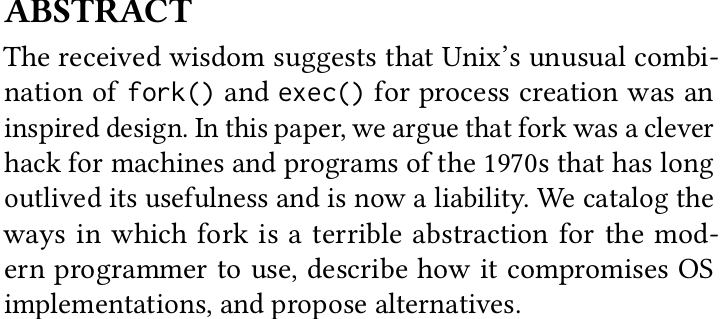
\includegraphics[width=5in]{../unix-api/fork-in-road-abs}
\end{frame}


\subsection{wait}

\againframe<5>{posixProcessFunctions}

\begin{frame}{wait/waitpid}
\begin{itemize}
\item \texttt{pid\_t waitpid(pid\_t pid, int *status, \\
              \hspace{5cm} int options)}
\item wait for a child process (with pid=\texttt{pid}) to finish
\item sets \texttt{*status} to its ``status information''
\vspace{.5cm}
\item \texttt{pid=-1} $\rightarrow$ wait for any child process instead
    \begin{itemize}
    \item \texttt{pid=0} almost the same
    \end{itemize}
\item options? see manual page (command \texttt{man waitpid})
    \begin{itemize}
        \item \texttt{0} --- no options
        %\item \myemph<2>{\texttt{WNOHANG}} --- return 0 rather than hanging if process not yet done
    \end{itemize}
\end{itemize}
\end{frame}

\begin{frame}[fragile,label=waitpidExample]{waitpid example}
\begin{lstlisting}[
    language=C++,
    style=smaller
]
#include <sys/wait.h>
...
  child_pid = fork();
  if (child_pid > 0) {
      /* Parent process */
      int status;
      waitpid(child_pid, &status, 0);
  } else if (child_pid == 0) {
      /* Child process */
      ...
\end{lstlisting}
\end{frame}



\subsection{summary diagram}

\usetikzlibrary{arrows.meta,decorations.pathmorphing,fadings}

\begin{frame}[fragile,label=typicalPatternSnake]{typical pattern}
\begin{tikzpicture}
\tikzset{
    thread/.style={very thick,draw,decorate,decoration=snake},
    split/.style={very thick,draw},
    marker/.style={thin,draw},
}
\path[thread] (0, 0) --  (0, -.5);
\node[anchor=south] at (0,0) {parent};
\node[anchor=north] (fork mark) at (0, -.5) {fork};
\draw[thread] (fork mark.south) -- (0, -2) node[below] (wait start) {waitpid};
\node (child start) at (9, -1.5) {child process};
\path[split] (fork mark) --  (child start);
\path[thread] (child start.south) -- (9, -2.5) node[below] (exec) {exec};
\path[thread] (exec.south) -- ++(0, -2) coordinate (exec done);
\path[marker] (exec done) -- ++(.5, 0) node[right] {exit()};
\path[split,dotted] (exec done) -- (0, -6);
\draw[very thick,dashed] (wait start) -- (0, -6);
\path[thread] (0, -6) -- ++(0, -3);
\end{tikzpicture}
\end{frame}


\begin{frame}[fragile,label=typicalPatternSnakeAlt]{typical pattern (alt)}
\begin{tikzpicture}
\tikzset{
    thread/.style={very thick,draw,decorate,decoration=snake},
    split/.style={very thick,draw},
    marker/.style={thin,draw},
}
\path[thread] (0, 0) --  (0, -.5);
\node[anchor=south] at (0,0) {parent};
\node[anchor=north] (fork mark) at (0, -.5) {fork};
\draw[thread] (fork mark.south) -- (0, -5.5) node[below] (wait start) {waitpid};
\node (child start) at (9, -1.5) {child process};
\path[split] (fork mark) --  (child start);
\path[thread] (child start.south) -- (9, -2.5) node[below] (exec) {exec};
\path[thread] (exec.south) -- ++(0, -1) coordinate (exec done);
\path[marker] (exec done) -- ++(.5, 0) node[right] {exit()};
\path[split,dotted] (exec done) -- (wait start.east);
%\draw[very thick,dashed] (wait start) -- (0, -6);
\path[thread] (wait start.south) -- ++(0, -3);
\end{tikzpicture}
\end{frame}

\begin{frame}[fragile,label=typicalPattern]{typical pattern (detail)}
\newcommand{\maincode}{
            pid = fork(); \\
            if (pid == 0) \{ \\
            \hspace{.5cm} exec\ldots(\ldots); \\
            \hspace{.5cm} \ldots \\
            \} else if (pid > 0) \{ \\
            \hspace{.5cm} waitpid(pid,\ldots); \\
            \hspace{.5cm} \ldots \\
            \} \\
            \ldots
}
\newcommand{\maincodeExec}{
            pid = fork(); \\
            if (pid == 0) \{ \\
            \hspace{.5cm} \myemph{exec\ldots(\ldots);} \\
            \hspace{.5cm} \ldots \\
            \} else if (pid > 0) \{ \\
            \hspace{.5cm} waitpid(pid,\ldots); \\
            \hspace{.5cm} \ldots \\
            \} \\
            \ldots
}
\newcommand{\maincodeWait}{
            pid = fork(); \\
            if (pid == 0) \{ \\
            \hspace{.5cm} exec\ldots(\ldots); \\
            \hspace{.5cm} \ldots \\
            \} else if (pid > 0) \{ \\
            \hspace{.5cm} \myemph{waitpid(pid,\ldots);} \\
            \hspace{.5cm} \ldots \\
            \} \\
            \ldots
}
\newcommand{\altcode}{
            main() \{ \\
            \hspace{.5cm} \ldots \\
            \} \\
}
\begin{tikzpicture}
\tikzset{
    code box/.style={draw,thick,font=\tt\fontsize{9}{10}\selectfont,align=left},
    with the code/.style={
        code box,
    },
    with the other code/.style={
        code box,
    }
}
\node[with the code] (start) {\maincode};
\node[with the code,anchor=north west] (parent first) at ([xshift=2cm,yshift=1cm]start.south east) {\maincodeWait};
\node[with the code,anchor=south west] (child first) at ([xshift=2cm,yshift=-1cm]start.north east) {\maincodeExec};
\node[with the other code,anchor=north west] (child second) at ([xshift=2cm]child first.north east) {\altcode};

\begin{scope}[very thick,>=Latex]
\draw[->] (start) -- (parent first);
\draw[->] (start) -- (child first);
\draw[->] (child first) -- (child second);
\end{scope}
\end{tikzpicture}
\end{frame}



\subsection{waiting for more than one?}


\usetikzlibrary{arrows.meta,decorations.pathmorphing,fadings}

\begin{frame}[fragile,label=patternMultSnake]{pattern with multiple?}
\begin{tikzpicture}
\tikzset{
    thread/.style={very thick,draw,decorate,decoration=snake},
    split/.style={very thick,draw},
    marker/.style={thin,draw},
}
\path[thread] (0, 0) --  (0, -.5);
\node[anchor=south] at (0,0) {parent};
\node[anchor=north] (fork mark 1) at (0, -.5) {fork};
\draw[thread] (fork mark 1) -- ++(0, -1) node[below] (fork mark 2) {fork};
\draw[thread] (fork mark 2.south) -- ++(0, -1) node[below] (wait 1 start) {waitpid(first,\ldots)};
\node (child 1 start) at (9, -1.5) {first child process};
\node (child 2 start) at (4, -2.5) {second child process};
\path[split] (fork mark 1) --  (child 1 start);
\path[split] (fork mark 2) --  (child 2 start);
\path[thread] (child 1 start.south) -- ++(0, -1) node[below] (exec 1) {exec};
\path[thread] (exec 1.south) -- ++(0, -2) coordinate (exec 1 done);
\path[marker] (exec 1 done) -- ++(.5, 0) node[right] {exit()};
\path[thread] (child 2 start.south) -- ++(0, -1) node[below] (exec 2) {exec};
\path[thread] (exec 2.south) -- ++ (0, -0.5) coordinate (exec 2 done);
\path[marker] (exec 2 done) -- ++(.5, 0) node[right] {exit()};
\path[split,dotted] (exec 1 done) -- (0, -6) coordinate (wait 1 done);;
\draw[very thick,dashed] (wait 1 start) -- (wait 1 done);
\draw[thread] (wait 1 done) -- ++(0, -.5) node[below] (wait 2 start) { waitpid(second,\ldots) };
\path[split,dotted] (exec 2 done) -- (wait 2 start);
\draw[overlay,thread] (wait 2 start.south) -- ++ (0, -2);
\end{tikzpicture}
\end{frame}


\againframe<6>{posixProcessFunctions}

\subsection{exercises (fork+exec+wait)}

\begin{frame}[fragile,label=fork-wait-ex1]{exercise (1)}
\vspace{-.25cm}
\begin{lstlisting}[basicstyle=\fontsize{9.5}{10.5}\tt\selectfont]
int main() {
    pid_t pids[2]; const char *args[] = {"echo", "ARG", NULL};
    const char *extra[] = {"L1", "L2"};
    for (int i = 0; i < 2; ++i) {
        pids[i] = fork();
        if (pids[i] == 0) {
            args[1] = extra[i];
            execv("/bin/echo", args);
        }
    }
    for (int i = 0; i < 2; ++i) {
        waitpid(pids[i], NULL, 0);
    }
}
\end{lstlisting}
\newcommand{\shownewline}{ {\fontsize{9}{10}\selectfont(newline)} }
Assuming fork and execv do not fail, which are possible outputs?
\begin{tabular}{llll}
\bfseries A. & \tt L1\shownewline L2 & \bfseries D. & A and B \\
\bfseries B. & \tt L1\shownewline L2\shownewline L2 & \bfseries E. & A and C \\
\bfseries C. & \tt L2\shownewline L1 & \bfseries F. & all of the above \\
    ~ &  ~ & \bfseries G. & something else \\
\end{tabular}
\end{frame}

\iftoggle{heldback}{\providecommand{\correct}[1]{#1}}{\providecommand{\correct}[1]{\myemph<2>{#1}}}

\begin{frame}[fragile,label=fork-wait-ex2]{exercise (2)}
\vspace{-.4cm}
\begin{lstlisting}[basicstyle=\fontsize{9.5}{10.5}\tt\selectfont]
int main() {
    pid_t pids[2]; const char *args[] = {"echo", "0", NULL};
    for (int i = 0; i < 2; ++i) {
        pids[i] = fork();
        if (pids[i] == 0) { execv("/bin/echo", args); }
    }
    printf("1\n"); fflush(stdout);
    for (int i = 0; i < 2; ++i) {
        waitpid(pids[i], NULL, 0);
    }
    printf("2\n"); fflush(stdout);
}
\end{lstlisting}
\newcommand{\shownewline}{ {\normalfont\fontsize{9}{10}\selectfont(newline)} }
Assuming fork and execv do not fail, which are possible outputs?
\begin{tabular}{llll}
\bfseries A. & \tt 0\shownewline 0\shownewline 1\shownewline 2 & \bfseries E. & \correct{A, B, and C} \\
\bfseries B. & \tt 0\shownewline 1\shownewline 0\shownewline 2 & \bfseries F. & C and D \\
\bfseries C. & \tt 1\shownewline 0\shownewline 0\shownewline 2 & \bfseries G. & all of the above \\
\bfseries D. & \tt 1\shownewline 0\shownewline 2\shownewline 0 & \bfseries H. & something else \\
\end{tabular}
\end{frame}

